%%%%%%%%%%%%%%%%%%%%%%%%%%%%%%%%%%%%%%%%%%%%%%%%%%%%%%%%%%%%%%%%%%%%%%%%%%%%%%%%%%%%%%%%%%%%%%%%
%
% CS484 Written Question Template
%
% Acknowledgements:
% The original code is written by Prof. James Tompkin (james_tompkin@brown.edu).
% The second version is revised by Prof. Min H. Kim (minhkim@kaist.ac.kr).
%
% This is a LaTeX document. LaTeX is a markup language for producing 
% documents. Your task is to fill out this document, then to compile 
% it into a PDF document. 
%
% 
% TO COMPILE:
% > pdflatex thisfile.tex
%
% If you do not have LaTeX and need a LaTeX distribution:
% - Personal laptops (all common OS): www.latex-project.org/get/
% - We recommend latex compiler miktex (https://miktex.org/) for windows,
%   macTex (http://www.tug.org/mactex/) for macOS users.
%   And TeXstudio(http://www.texstudio.org/) for latex editor.
%   You should install both compiler and editor for editing latex.
%   The another option is Overleaf (https://www.overleaf.com/) which is 
%   an online latex editor.
%
% If you need help with LaTeX, please come to office hours. 
% Or, there is plenty of help online:
% https://en.wikibooks.org/wiki/LaTeX
%
% Good luck!
% Min and the CS484 staff
%
%%%%%%%%%%%%%%%%%%%%%%%%%%%%%%%%%%%%%%%%%%%%%%%%%%%%%%%%%%%%%%%%%%%%%%%%%%%%%%%%%%%%%%%%%%%%%%%%
%
% How to include two graphics on the same line:
% 
% \includegraphics[width=0.49\linewidth]{yourgraphic1.png}
% \includegraphics[width=0.49\linewidth]{yourgraphic2.png}
%
% How to include equations:
%
% \begin{equation}
% y = mx+c
% \end{equation}
% 
%%%%%%%%%%%%%%%%%%%%%%%%%%%%%%%%%%%%%%%%%%%%%%%%%%%%%%%%%%%%%%%%%%%%%%%%%%%%%%%%%%%%%%%%%%%%%%%%

\documentclass[11pt]{article}

\usepackage[english]{babel}
\usepackage[utf8]{inputenc}
\usepackage[colorlinks = true,
            linkcolor = blue,
            urlcolor  = blue]{hyperref}
\usepackage[a4paper,margin=1.5in]{geometry}
\usepackage{stackengine,graphicx}
\usepackage{fancyhdr}
\setlength{\headheight}{15pt}
\usepackage{microtype}
\usepackage{times}
\usepackage{float}

% From https://ctan.org/pkg/matlab-prettifier
\usepackage[numbered,framed]{matlab-prettifier}

\frenchspacing
\setlength{\parindent}{0cm} % Default is 15pt.
\setlength{\parskip}{0.3cm plus1mm minus1mm}

\pagestyle{fancy}
\fancyhf{}
\lhead{Homework 5 Questions}
\rhead{CS484}
\rfoot{\thepage}

\date{}

\title{\vspace{-1.5cm}Homework 5 Questions}


\begin{document}
\maketitle
\vspace{-3cm}
\thispagestyle{fancy}

\section*{Instructions}
\begin{itemize}
  \item 3 questions.
  \item Write code where appropriate.
  \item Feel free to include images or equations.
  \item Please make this document anonymous.
  \item \textbf{Please use only the space provided and keep the page breaks.} Please do not make new pages, nor remove pages. The document is a template to help grading. If you need extra space, please use and refer to new pages at the end of the document.
\end{itemize}

\section*{Questions}

\paragraph{Q1:} Given a linear classifier, how might we handle data that are not linearly separable? How does the \emph{kernel trick} help in these cases? (See course slides in supervised learning, plus your own research.)

%%%%%%%%%%%%%%%%%%%%%%%%%%%%%%%%%%%
\paragraph{A1:} The kernel trick helps us to separate data that are not linearly separable. It uses a mapping function called the kernel to transform the given space to a space of usually very high dimension. The idea is that if the data is not linearly separable in our \emph{n} dimensional space, it may be separable in a higher dimension. An example of kernel transformation is shown in the figure below.
\begin{figure}[H]
	\centering
	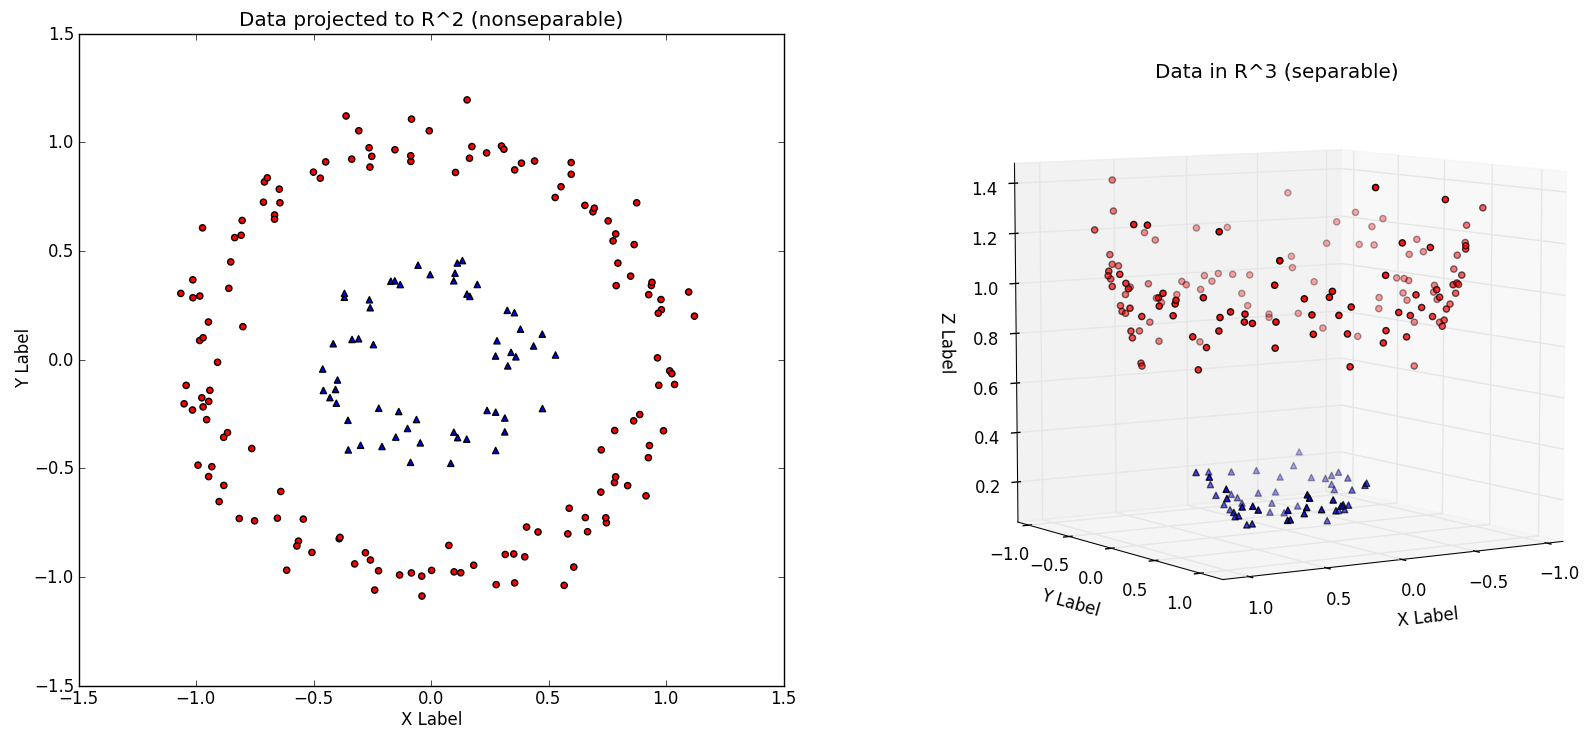
\includegraphics[width=0.8\textwidth]{kernel_trick.png}
	\label{fig:kernel}
\end{figure}



%%%%%%%%%%%%%%%%%%%%%%%%%%%%%%%%%%%

\pagebreak
\paragraph{Q2:} In machine learning, what are bias and variance? When we evaluate a classifier, what are overfitting and underfitting, and how do these relate to bias and variance?

%%%%%%%%%%%%%%%%%%%%%%%%%%%%%%%%%%%
\paragraph{A2:} The bias error occurs from erroneous assumption in the learning algorithm. It is the difference between the prediction and the true value. Underfitting occurs when the model cannot adequately capture the underlying structure of the data. In underfitting, the bias error is high and the algorithm misses the relevant relations between features and target outputs. The variance is the sensitivity to small fluctuations in the training data. Overfitting occurs when the model matches the data too closely that it is likely to fail in additional data. When variance is high, the model matches the random noise in the training data as well, also known as overfitting. 



%%%%%%%%%%%%%%%%%%%%%%%%%%%%%%%%%%%

% Please leave the pagebreak
\pagebreak
\paragraph{Q3:} The way that the bag of words representation handles the spatial layout of visual information can be both an advantage and a disadvantage. Describe an example scenario for each of these cases, plus describe a modification or additional algorithm which can overcome the disadvantage. 

How might we evaluate whether bag of words is a good model?

%%%%%%%%%%%%%%%%%%%%%%%%%%%%%%%%%%%
\paragraph{A3:} The bag of words method ignores the spatial relationships among the patches, but it can be important in an image representation. Such limitation can be overcome by including the spatial information into the algorithm. For example, the image can be divided into increasingly smaller sub-regions and compute local histograms in each sub-region as the pyramid matching approach. Also, the augmentation of SIFT by their spatial coordinates can introduce spatial information to the bag of words model. Although it does not consider the spatial relationship between patches, it is an intuitive way of classifying images based on the frequency of each visual words if they have unique words in each image. The bag of words model is commonly evaluated using the confusion matrix. 



%%%%%%%%%%%%%%%%%%%%%%%%%%%%%%%%%%%

% If you really need extra space, uncomment here and use extra pages after the last question.
% Please refer here in your original answer. Thanks!
%\pagebreak
%\paragraph{AX.X Continued:} Your answer continued here.



\end{document}
